
%%%%%%%%%%%%%%%%%%%%%%% file typeinst.tex %%%%%%%%%%%%%%%%%%%%%%%%%
%
% This is the LaTeX source for the instructions to authors using
% the LaTeX document class 'llncs.cls' for contributions to
% the Lecture Notes in Computer Sciences series.
% http://www.springer.com/lncs       Springer Heidelberg 2006/05/04
%
% It may be used as a template for your own input - copy it
% to a new file with a new name and use it as the basis
% for your article.
%
% NB: the document class 'llncs' has its own and detailed documentation, see
% ftp://ftp.springer.de/data/pubftp/pub/tex/latex/llncs/latex2e/llncsdoc.pdf
%
%%%%%%%%%%%%%%%%%%%%%%%%%%%%%%%%%%%%%%%%%%%%%%%%%%%%%%%%%%%%%%%%%%%


\documentclass[runningheads]{llncs}

\usepackage{amssymb}
\setcounter{tocdepth}{3}
\usepackage{graphicx}
\usepackage{caption}
\usepackage{pdfpages}
\usepackage[]{algorithm2e}
\usepackage[]{listings}
\usepackage{geometry}
 \geometry{
bottom = 25 mm
 }
 \usepackage{color}
 
\definecolor{codegreen}{rgb}{0,0.6,0}
\definecolor{codegray}{rgb}{0.5,0.5,0.5}
\definecolor{codepurple}{rgb}{0.58,0,0.82}
\definecolor{backcolour}{rgb}{0.95,0.95,0.92}
 
\lstdefinestyle{mystyle}{
    backgroundcolor=\color{backcolour},   
    commentstyle=\color{codegreen},
    keywordstyle=\color{magenta},
    numberstyle=\tiny\color{codegray},
    stringstyle=\color{codepurple},
    basicstyle=\footnotesize,
    breakatwhitespace=false,         
    breaklines=true,                 
    captionpos=b,                    
    keepspaces=true,                 
    numbers=left,                    
    numbersep=5pt,                  
    showspaces=false,                
    showstringspaces=false,
    showtabs=false,                  
    tabsize=2
}
 
\lstset{style=mystyle}



\usepackage{url}
\urldef{\mailsc}\path|rahmank@purdue.edu|    
\newcommand{\keywords}[1]{\par\addvspace\baselineskip
\noindent\keywordname\enspace\ignorespaces#1}

\begin{document}

\mainmatter  % start of an individual contribution

% first the title is needed
\title{Reducing Consistency While Keeping Correctness Using SAT Solvers}

% a short form should be given in case it is too long for the running head
\titlerunning{}

% the name(s) of the author(s) follow(s) next
%
% NB: Chinese authors should write their first names(s) in front of
% their surnames. This ensures that the names appear correctly in
% the running heads and the author index.
%
\institute{Kiarash Rahmani\\
\mailsc\\
\url{https://github.com/Kiarahmani/CAPR2016}}

\author{Computer-Aided Program Reasoning Course Project - Dr. Samanta }
%
\authorrunning{CAPR2016 - Course Project}
% (feature abused for this document to repeat the title also on left hand pages)

% the affiliations are given next; don't give your e-mail address
% unless you accept that it will be published


%
% NB: a more complex sample for affiliations and the mapping to the
% corresponding authors can be found in the file "llncs.dem"
% (search for the string "\mainmatter" where a contribution starts).
% "llncs.dem" accompanies the document class "llncs.cls".
%

\toctitle{Lecture Notes in Computer Science}
\tocauthor{Authors' Instructions}
\maketitle


\begin{abstract}
As a result of the CAP theorem, today's distributed databases offer various levels of \emph{weak consistency}. Application developers must pick the correct consistency level for each operation to preserve the correctness of their application. Recent  works\cite{quelea} successfully take this burden off the developer's shoulders. They correctly choose the weakest store offered consistency, that preserves application-level requirements. We are now planning to extend these works by actually {\bf implementing} required consistency guarantees.

\keywords{Eventual Consistency, SAT solvers, Synthesis, Weak Consistency, Quelea, Cassandra }
\end{abstract}

\section{Introduction}
\paragraph{}
Replication is a must in the real-world web services such as those maintained by Facebook, Google or Twitter. These systems replicate data and logic across geo-distributed data centers (and also within data centers) to reduce user-perceived latency and to tolerate network partitioning and node failures. 
\\
As the running example, let's consider a replicated bank account software, that serves the clients via the host data center.  In an ideal world, clients would submit request to the local replica, updates are created locally and \emph{ would become available at all other replicas immediately}. However, we know this is not the case in reality: physical network partitions are unavoidable and delay in update propagation is non-negligible.\\ It is easy to see why this can become problematic, if replicas do not synchronize operation execution:
\begin{center}
 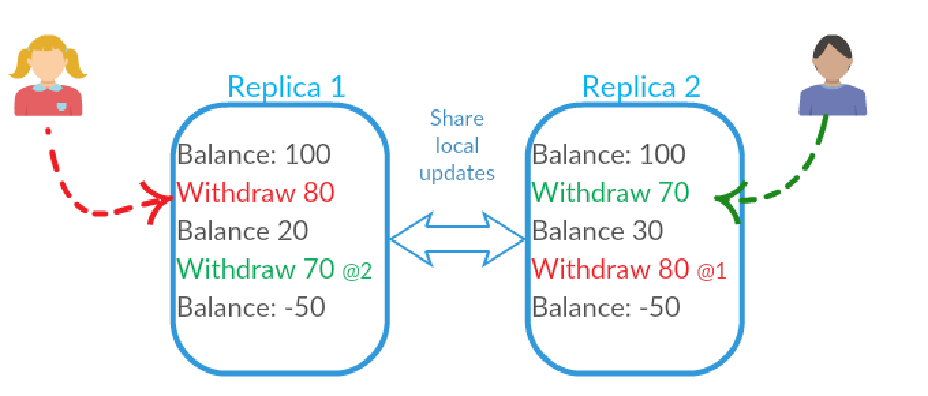
\includegraphics[scale = 0.6]{Anom1.pdf}
 \end{center} 
If two users concurrently submit updates on the same replicated object (for example, in the above figure the green transaction was submitted at replica 2 before the updates from red transaction became available at replica 2), the system might become inconsistent. 
This is due to the \emph{dependency of operations to the ordered history of updates available at that replica}\footnote {Some limited techniques can eliminate this dependency, look at \cite{crdt}}. For example, the Withdraw operation in the bank account, reads the current history of updates and decides if the money should be deducted or not. 
\paragraph {\bf Weak Consistency Levels:}
Above examples demonstrate the need for synchronization between replicas. However, always keeping the replicated data completely consistent, requires global consensus and massive communication between data stores, which reduces the overall performance. One might ask, is it even necessary in all cases to guarantee {\bf S}trong {\bf C}onsistency for all operations? 
Strong Consistency guarantees that read operations always return the most recent data regardless of which node delivers the data, however, is that really necessary?
For example, in the bank account example, we can permit the Deposit operations to perform and commit locally and the application still would be safe. In other words concurrent deposits cannot falsify the correctness of the bank account application. 
\\ In the above setting, the least thing that we must be sure of is that \emph{all updates become available at all replicas eventually}. 
This is called {\bf E}ventual {\bf C}onsistency and is usually offered by the underlying system. In general, any use cases in which providing an answer is more important than providing the most up-to-date answer can be served well by Eventual Consistency.
\\{\bf Weak Abstract Consistency} levels are those that fill the gap between EC and SC guarantees.
For example, {\bf C}ausal {\bf C}onsistency, guarantees that if an update is present in the replica, all updates that it witnessed at the time of execution -possibly at some other replica- are also present. In other words, two events that are ?causally?
related must appear in the same order at all nodes. Or {\bf R}ead {\bf M}y {\bf W}rites, guarantees that an operation always witnesses all the previous updates from its own session. 
\\ In a nutshell, at the program level, we want to be able to specify some sort of dependencies between events and expect the underlying system to preserve their order at all replicas. Consider the following two events; I -really- have to be sure that, \emph{at all replicas} the first event is executed before the second one:
\[ \textrm {[Removes professor from friends list]}\]
\[{\textrm [Posts]} \rightarrow  \textrm {"My teacher is the worst, I need to drop this course!" }\]
 

\section{Problem Definition}
\paragraph{}
Real world data-stores, do not offer any of the conceptually defined weak guarantees such as RMW or CC. They only let the users work with low-level notions like TWO (A write must be written on at least two node). As we can see there is a large conceptual gap here: the application writer only cares about the high-level invariant of the program (non-negative balance, for instance), but has to pick store-offered, low-level guarantees for each operation.
\begin{center}
\includegraphics[scale = 0.385]{gap.pdf}
\end{center}

As explained earlier this gap is filled by conceptual guarantees like CC, that offer one level of abstraction for the application writers: now users can pick one of these more abstract guarantees that have been previously implemented on top of the store. We call them more abstract, because they consider updates and relationships among them, as opposed to low-level inter replica agreements.
\begin{center}
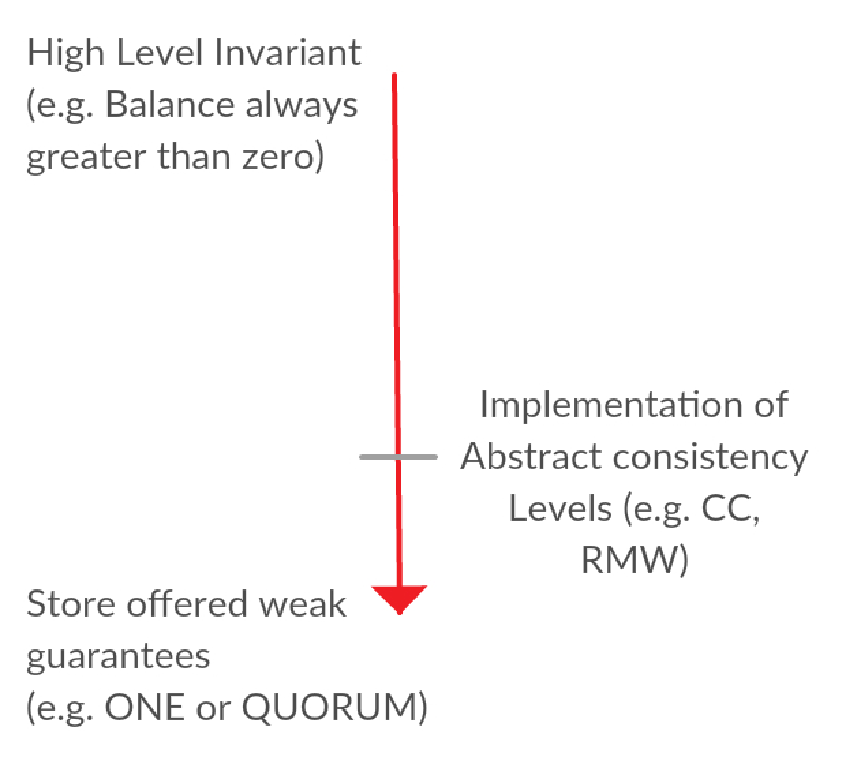
\includegraphics [scale = 0.38]{Gap1.pdf} \hspace{11 mm}
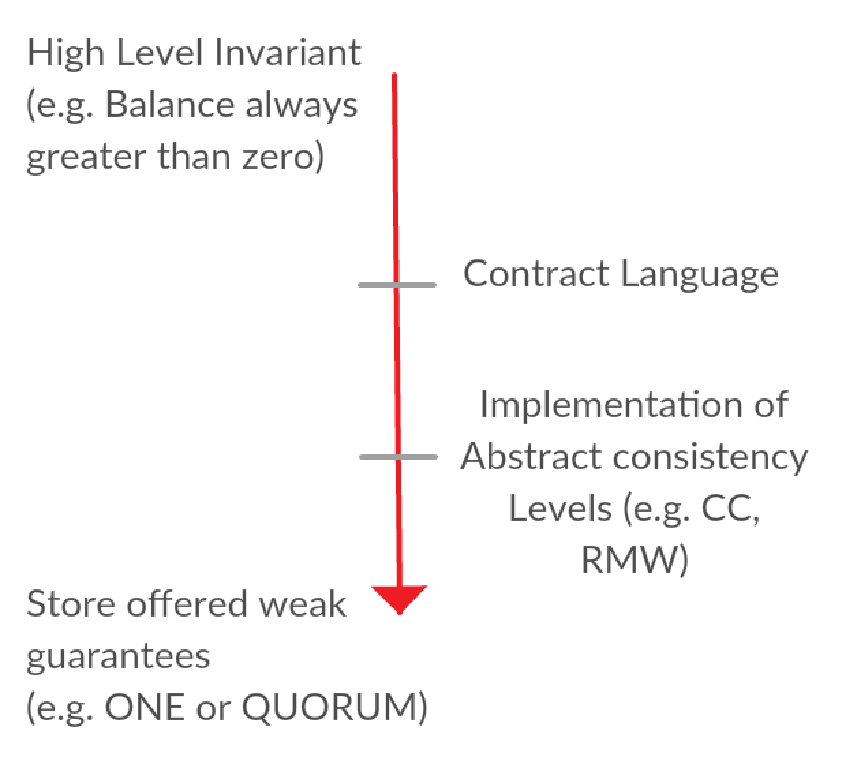
\includegraphics [scale = 0.38]{Gap2.pdf}
\end{center}

Recent developments, offer another level of abstraction: using a language of {\bf contracts}, user can specify the \emph{application level requirements} for each operations, and operations are automatically mapped to the correct available consistency implementation. For example following contract is mapped to CC: 
$$\forall (a:deposit) (b:withdraw). 
 ((vis(a,b))\wedge(vis(b,\eta)) \Rightarrow (vis(a,\eta)))$$
It simply says that if the current operation $\eta$ witnesses an update $b$, and $b$ has witnessed another update $a$, it must be the case that $\eta$ also witnesses $a$. 

\paragraph{}
This obviously makes the developers job easier, since he or she does not have to deal with the  low-level consistency guarantees anymore. \\However, there are still some problems remained...

\paragraph {\bf Current System and Proposed Extension}
Current system, based on the given contract \emph{maps} each operation to some \emph{pre-implemented} consistency level. Since the mapped level must preserve the contract's requirements, the system tends to be conservative: If $L1$ does not preserve the contract for the operation $op$ but $L2$ does, $op$ must be mapped to $L2$. However, $L2$ might be too strong for $op$ and we lose performance because of unnecessary synchronization. \\ \emph{ What if we could first analyze the code and the contracts and automatically synthesis the consistency levels that offer the exact guarantees required for each operation. }
\begin{center}
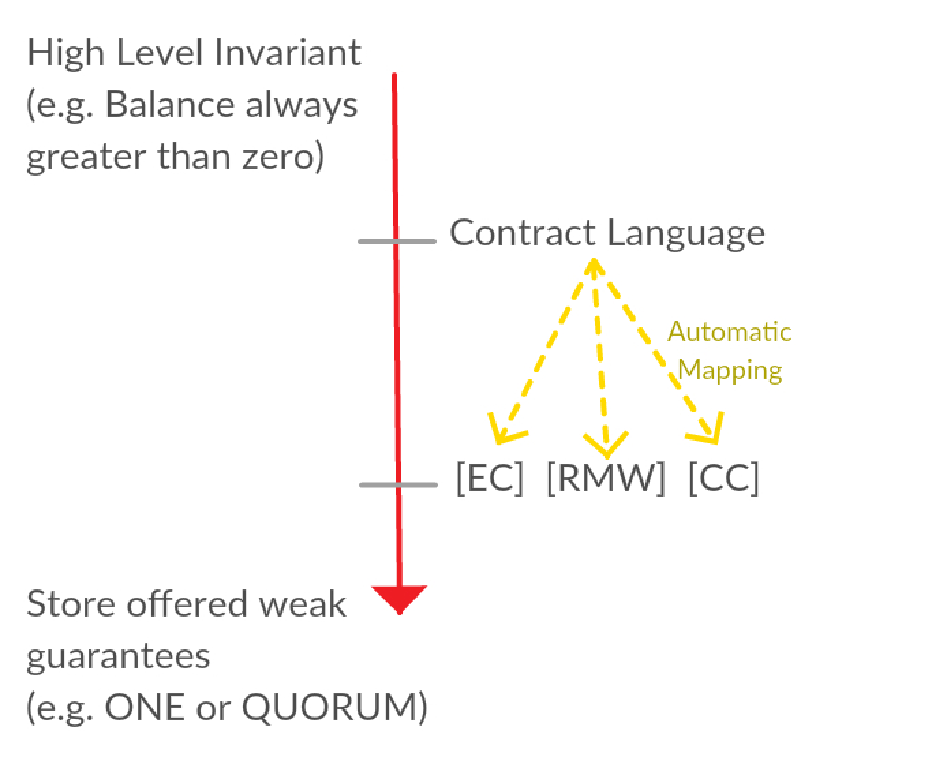
\includegraphics[scale=0.43]{Gap3.pdf} \hspace{7mm}
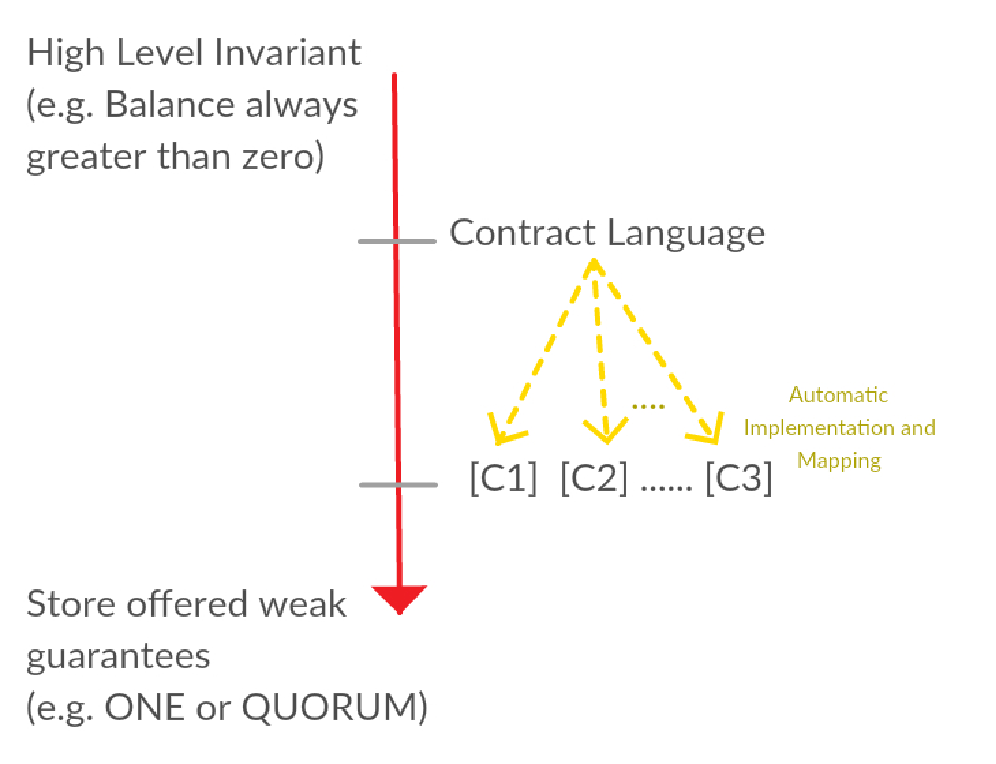
\includegraphics[scale=0.43]{Gap5.pdf}
\end{center}

\section{Proposed Approach}
\paragraph{\bf Well-Formed Contracts:}
Our first observation is that we can limit the structure of the contracts, without losing any generality. 
All interesting contracts can in fact, be written in the following form: 
\[\forall a, \Phi_{pre} \Rightarrow vis (a,\eta) \]
which specifies that, all updates that satisfy the pre-condition $\Phi_{pre}$ must be visible to the current operation $\eta$. This intuitively makes sense, since developer is only interested in specifying what updates must be witnessed by the operation that is being executed. 

\paragraph{\bf Cache Synthesis:} 
Our idea is to first analyze the contracts and create multiple caches on top of the store, each of which is guaranteed to show the specified behavior by the contract. For example if the contract of an operation is: \(\forall a, so(a,\eta) \Rightarrow vis(a,\eta)\), a cache is created for this contract that makes sure that the operation is executed only if $so^{-1}(\eta)$ is present in the cache (can be done by blocking the execution, until the required updates become available). For this project I am focusing on the important problem of figuring out the maximal set of events that the current operation can see, without falsifying user-defined correctness.
\subsection{First Steps}
We observed that contracts can be divided into two major groups and we deal with each separately: 
\paragraph{Wait-Free Contracts:} are those that never require blocking the operation: the cache can pick some subset of the available update and make only them visible to the current operation. For example, consider the following contract and its associated graph:
\[\forall a. vis (a,b) \wedge vis (b,\eta) \Rightarrow vis (a,\eta)\]
\begin{center}
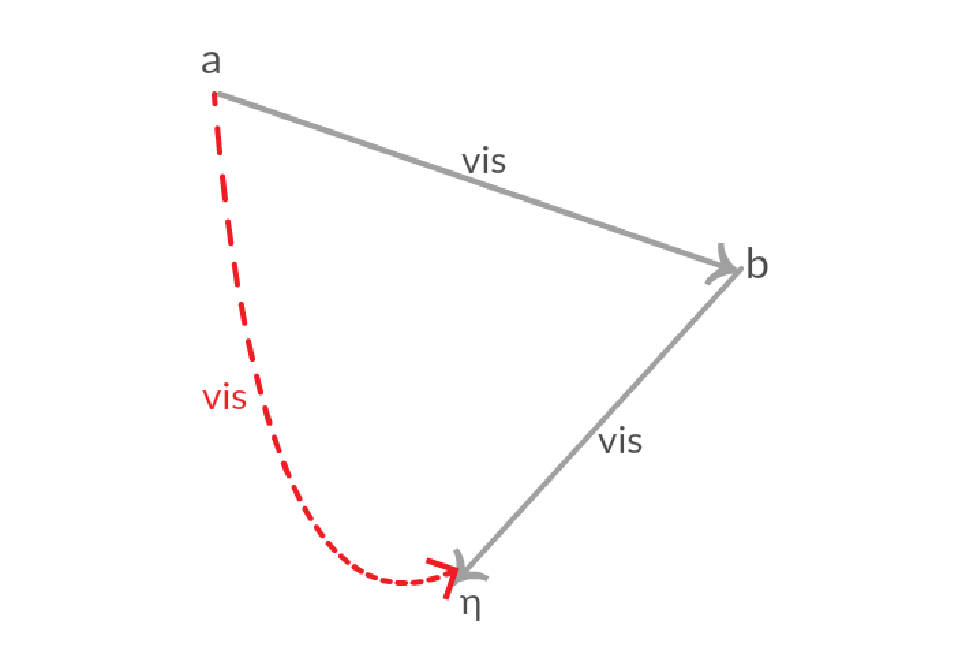
\includegraphics[scale=0.35]{c.pdf}
\end{center}
The contract specifies that if an effect $b$ is visible to the current operation,  all updates $a$ that were visible to $b$, must also be visible to the current operation. However, this does not mean the current operation must be blocked until all such updates are received: we can filter those $b$s that does not satisfy this property and then execute the current operation. In other words, we by filtering some present updates at the replica, the current operation can see a \emph {safe environment}  based on its contract. 
\\ The important property that our filter must have, is called MAX-VIS and is defined as follows: \\
\emph{if the cache filters out some updates and returns $S$ as the safe environment, there cannot be an update $u$ in the store, that $S\cup \{u\}$ is safe}.

\vspace{5mm}
\paragraph{Waiting Contracts:}
Similarly, there are some contracts, that when implemented in the cache, waiting for some updates would be unavoidable:
\[\forall a. so(a,\eta) \Rightarrow vis(a,\eta)\]
\begin{center}
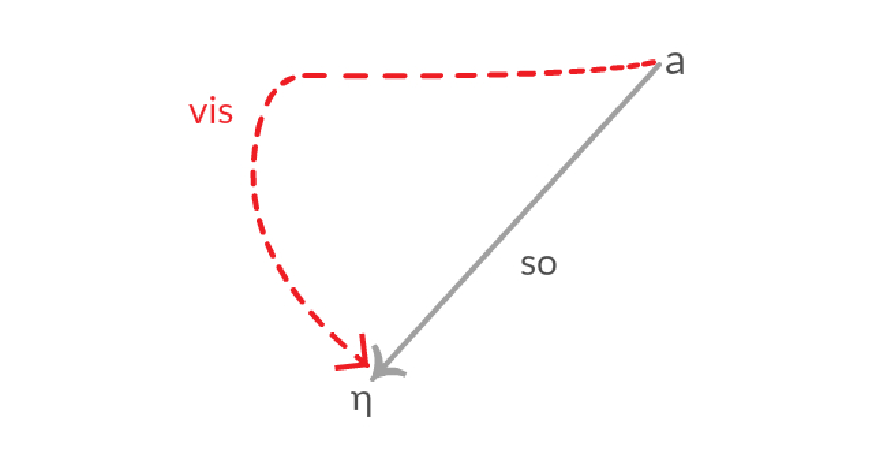
\includegraphics[scale=0.4]{c1.pdf}
\end{center}
This specifies that every previous update in the same session with the current operation, must be visible to this operation. This means that the current operation must be blocked until those updates become available at the local replica. Similar to the previous section, we define MIN-WAIT property for the blocking, as follows:
\\ \emph{if cache blocks the current operation, until a set $s$ of updates are arrived, there cannot be a smaller set $s'$, that $R\cup\{s'\}$ is safe (R is the effects available at the replica). }


\subsection {Contract Analysis}
\paragraph{} 
By analyzing the associated graph for each contract, we realized that for all the wait-free contracts, the pre-condition part (gray section in the figures) ends with a $vis$ edge pointing to the current operation. This intuitively makes sense, because a $vis$ edge brings flexibility to the system: we can manipulate the pre-condition of the contract, by modifying the set of effects that are visible to the current operation. On the other hand, Waiting contracts always have an $so$ edge pointing to the current operation: $so$ is the session order relation, which cannot be modified by the system; as a result pre-condition cannot be changed and wait is unavoidable. 

\begin{figure}
\centering
\begin{minipage}{.5\textwidth}
  \centering
  \includegraphics[width=.6\linewidth]{c2.pdf}
  \captionof{figure}{Wait-Free Contracts}
  \label{fig:test1}
\end{minipage}%
\begin{minipage}{.5\textwidth}
  \centering
  \includegraphics[width=.6\linewidth]{c3.pdf}
  \captionof{figure}{Waiting Contracts}
  \label{fig:test2}
\end{minipage}\end{figure}

As mentioned previously, for wait-free contracts we need to find out what subset of available effects must be made visible to the current operation, and for the waiting contracts the operation must be blocked until the minimal set of required effects become available. Our synthesis is nothing but a shim layer on top of the actual database that figures out the visibility set for the current operation or possibly blocks it until all dependencies are available. Thus the main theoretical question we need to answer is how to find out the maximal \emph{visibility} and minimal \emph{wait-for}  sets. 

\subsection{From Contract to SAT Formula - An Example}
Let's start with a concrete example. Assume we have the following local setting: 5 effects are available at the replica whose visibility sets are recorded. For example, effect A at the time of execution has witnessed three effects: \(\{x,y,z\}\).
Now an operation \(op\) is submitted to the replica whose consistency guarantee is given by the following contract: 
$(vis(a,b))\wedge(vis(b,\eta)) \Rightarrow (vis(a,\eta))$. Since this is a wait-free contract, there is no need to block \(op\). However, the shim must automatically figure out what subset of \(\{x,y,A,B,C\}\) is safe to be shown to \(op\). \begin{center}
\includegraphics[scale=1]{c4.pdf}
\end{center}
For this easy example, we can see that the maximal visibility set for \(op\) is \(\{x,y,B\}\); because if we include \(A\) in the visibility set, that means \(vis(A,\eta)\) holds, and since \(vis(z,A)\) also holds, based on \(op\)'s contract, \(vis (z,\eta)\) must also hold, which is not the case because \(z\) is not available at the replica yet. Moreover, since \(A\) is not in the visibility set, with a similar reasoning \(C\) also cannot be included. \\
We successfully, translated this problem into a Max-SAT problem as follows: Find an assignment for each variable that satisfies the following hard constraints and maximizes the number of soft constraints. All variables that are assigned true must be included in the visibility set. \\
\begin {center}
\includegraphics[scale=0.5]{c6.png}\\
\end{center}
The soft constraints clearly represent the presence of the effects in the visibility set, and the hard constraints are built from this particular example's contract. Each line represents constraints on one of the effects: z is not available yet, so it cannot be True, \(x\) and \(y\) have no constraint because their original visibility sets were empty. For the rest, each clause represents one visibility relation that according to the contract must be satisfied. For example, the only clause for effect \(C\), clearly states that either \(C\) must not be true, or \(A\) must also be true (= present). 

\subsection {SAT Formula Generator}
Here we explain an algorithm to craft a Max-SAT instance similar to the previous example, given a contract. For the sake of simplicity, here we explain the algorithm for a simpler and more restricted type of contracts. We only consider contracts in which each effect appears only in at most two relations - i.e. no multi-edge node in the associated graph. We believe that our approach can easily be extended to support multi-edge graphs.

\begin{center}
\includegraphics[scale=0.73]{c7.pdf} 
\end{center}

Our algorithm is a simple graph traversal that starts from \(\eta\) and goes up until reaches the last node before the red \(vis\) edge.  Starting from the base node, at each iteration, it covers one edge and computes the set for the next node and repeats for all edges. Later it computes the hard and soft constraints based on these sets: the soft constraints are always the conjunction of all present effects at the replica, but hard constraints are modified at each iteration. 
\\ \\ \\ \\ \\

\begin{lstlisting}[language = Java , caption= Algorithm Sketch, escapeinside={*(}{*)}]
Input: list of edges [E_1, E_2, .... , E_k]; set A of available effects
Output: Mapping from effects to sets of Clauses. 
--------------------------------------------------------------------------
H[1] = A; 
for (i in [1...k-1])
	if (E_i.type() == vis)
		H[i+1] = union of visibility sets of all effects in H[i] 
		
	else if(E_i.type() == so)
			H[i+1] = union of in-session precedents of all effects in H[i]
			
//Now list H contains all effects at each node that satisfy the relation to the base effect at that node specified by the subgraph.	

for (i in [1...k-1])
	if (E_i.type() == vis){
		for effect e in H[i]
			if (e is present in the replica)
				for all a in e.visibility()
					add clause (not e \/ a) to the hard constraints of e
			else
				add (not e)			
	}
	else if(E_i.type() == so)
		for effect e in H[i]
			if (e is present in the replica)
				for all a in e.session_order()
					add clause (not e \/ a) to the hard constraints of e
			else
				add (not e)	
\end{lstlisting}

Note that this is not a precise algorithm yet. However, we manually computed the Max-SAT formula for a number of simple contracts and the algorithm seems right. In a nutshell, it just traverses the graph upward, and at each step figures out all effects that satisfy the relation given by the traversed subgraph to the base effect \(\eta\). When covering an edge of type \(r\), for each of the effects e present at the set associated with the current node,
 it finds out all effects \(a\) that satisfy relation \(r\) with \(e\),  and adds a clause to the hard constraints of \(e\). The clause is of the form \((\neg e \vee a)\) which obviously states that if e is going to be present (i.e is true), a must also be present. 
 
 \subsection{next steps?}
 We already have a reduction algorithm from finding max-vis set to max-SAT. Of course, it needs to be generalized to support all sorts of graphs and then implemented. The synthesizer must take a contract and return a function F. Function F is a black-box in our tool that magically (actually, after calling the SAT solver) tells us what subset of the available effects at the replica must be made visible to the current operation. 
 \paragraph{}
 I believe the rest of the project will be dedicated to the implementation of these ideas in a packed tool that would hopefully show reasonable performance, while preserving fine-grained guarantees requested by the user.
 





\begin{thebibliography}{4}


\bibitem{quelea} KC Sivaramakrishnan, G. Kaki, S. Jagannathan: Declarative Programming over
Eventually Consistent Data Stores. PLDI '15. 

\bibitem{crdt} M. Shapiro, N. Pregui�a, C. Baquero, M. Zawirski : A comprehensive study of Convergent and Commutative Replicated Data Types. RR-7506, INRIA. 2011, pp.50. 



\bibitem{rdt} S. Burckhardt et. al: Replicated Data Types: Specification, Verification, Optimality. POPL'14.


\bibitem{bc} S. Gilbert, N. Lynch: Brewer's conjecture and the feasibility of
consistent, available, partition-tolerant web services. SIGACT News,
33(2):51-59, June 2002. 

\bibitem{chapar} M. Lesani, C. Bell, A. Chlipala: Chapar: Certified Causally Consistent
Distributed Key-Value Stores. POPL'16.

\bibitem{dynamo} G.DeCandia et.al. : Dynamo: Amazon's Highly Available Key-value Store. SOSP'07.



\end{thebibliography}
\end{document}
